\documentclass[fullscreen=true,unicode,bookmarks=true,colorlinks,urlcolor=blue,unicode]{beamer}

\usepackage{ofvp_beamer_packages} % Дополнительные пакеты для презентации и PDF для МЛЦ

\usepackage{ofvp_beamer_theme} % Тема презентаций для МЛЦ

\title{Сравнительный анализ параллельных численных алгоритмов решения нелинейного уравнения квазиоптики}
\author[Дергачёв А.\,А., Ефимов О.\,В., Сметанина Е.\,О.]{Дергачёв А.\,А., \underline{Ефимов О.\,В.}, Сметанина Е.\,О.}
\institute[МГУ имени М.\,В. Ломоносова]{
			Московский государственный университет имени М.\,В. Ломоносова\\
			Физический факультет, кафедра общей физики и волновых процессов\\
			Международный учебно-научный лазерный центр\\
			НОЦ <<Суперкомпьютерные технологии>>\\
}
\date[2009]{14 декабря 2009}

% PDF settings
\hypersetup{
	pdftitle={Сравнительный анализ параллельных численных алгоритмов решения нелинейного уравнения квазиоптики},
	pdfauthor={Дергачёв А. А., Ефимов О. В., Сметанина Е. О.},
	pdfsubject={Сравнительный анализ параллельных численных алгоритмов решения нелинейного уравнения квазиоптики},
	pdfkeywords={параллельные алгоритмы, нелинейное уравнение квазиоптики, эффективность распараллеливания, быстрое преобразование Фурье}
}

% For graphics/media
\def\imagesdir{../images}
\def\graphsdir{../graphs_color}
\def\moviesdir{./video}

\begin{document}

	\begin{frame}
		\titlepage
	\end{frame}


	\section{Введение}

	\subsection{Филаментация}
	
	\begin{frame}
		\frametitle{Приложения филаментации}
		
		\begin{columns}[c,totalwidth=\textwidth]
			\column[c]{0.7\textwidth}	
				\begin{itemize}
					\item Экологический мониторинг атмосферы \\
							{\scriptsize \color{gray} \hspace{2em} широкий спектр суперконтинуума}
					\item Удаленное зондирование мишеней \\
							{\scriptsize \color{gray} \hspace{2em} высокая интенсивность}
					\item Управляемый газовый разряд \\
							{\scriptsize \color{gray} \hspace{2em} высокая линейная плотность плазмы}
					\item Микро-модификация оптических материалов \\
							{\scriptsize \color{gray} \hspace{2em} малый размер филамента \\
							\hspace{2em} высокая интенсивность}
				\end{itemize}
				
				\begin{centering}
        			\begin{figure}
           				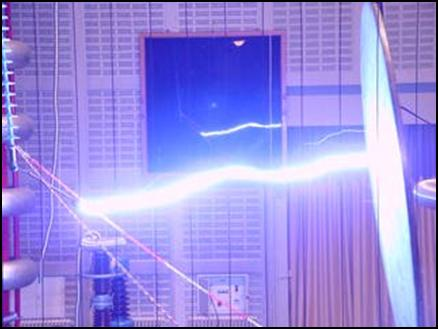
\includegraphics[width=0.3\textwidth]{\imagesdir/applications2_1.jpg}
           				\hspace{3.0em}
           				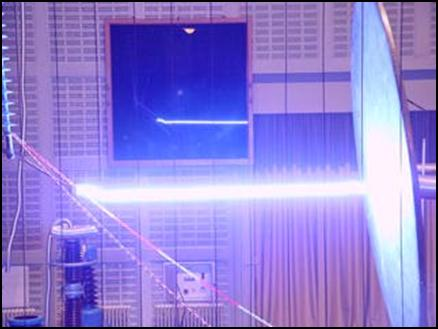
\includegraphics[width=0.3\textwidth]{\imagesdir/applications2_2.jpg}
        			\end{figure}
				\end{centering}
			\column[c]{0.3\textwidth}				
	        		\begin{figure}
	           			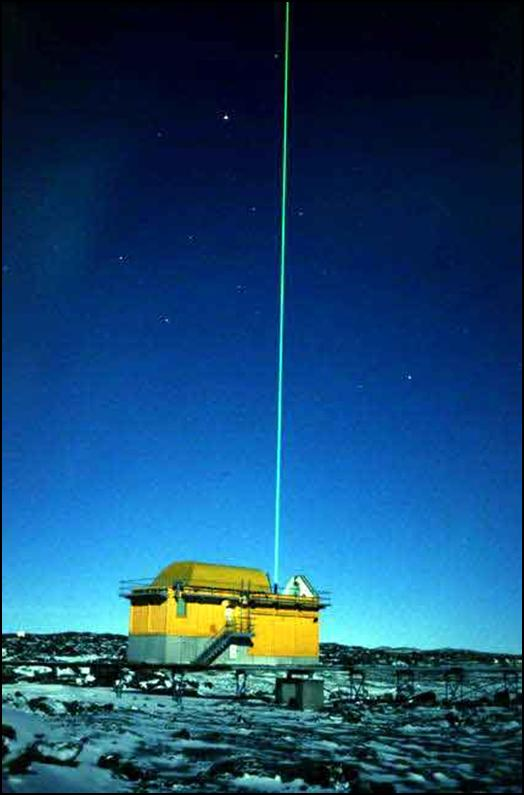
\includegraphics[width=0.8\textwidth]{\imagesdir/applications1.jpg} \\
	           			\vspace{1.0em}
	           			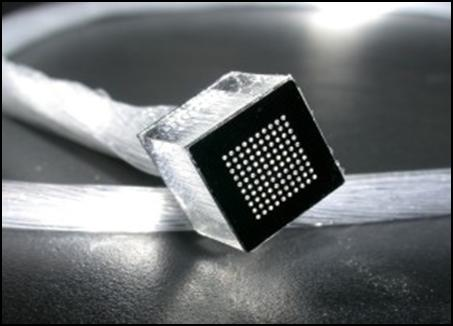
\includegraphics[width=0.8\textwidth]{\imagesdir/applications3.jpg}
	        		\end{figure}
		\end{columns}
	\end{frame}
	
	
	\section{Математическая модель}

	\subsection{Рассматриваемое уравнение и начальные условия}

	\begin{frame}
		\frametitle{Постановка задачи}

		\only<1>{
			Параболическое уравнение квазиоптики:
			\begin{equation*}
				2\textbf{i}k\dfrac{\partial E}{\partial z} = \Delta_{\perp}E + \frac{2k^2}{n_0}n_2|E|^2 E
			\end{equation*}
			
			Начальные условия:
			\begin{equation*}
				E(x, y, z = 0) = E_0 \exp\left( -\dfrac{x^2 + y^2}{2 r_0^2} \right)
			\end{equation*}
		}
		
		\only<2>{
			Обезразмеренная задача:
			\begin{equation*}
				\left\{
					\begin{array}{l}
						2\textbf{i}\dfrac{\partial E}{\partial z} = \Delta_{\perp} E + R |E|^2 E \\
						E(x, y, z = 0) = \exp\left( -\dfrac{x^2 + y^2}{2} \right) \\
					\end{array}
				\right.
			\end{equation*}
		}
	\end{frame}


	\section{Численные методы решения задачи}

	\subsection{Общее описание}
	
	\begin{frame}
		\frametitle{Численные методы решения задачи}

			\begin{itemize}
			\item Явная разностная схема: метод Рунге-Кутта \\
					{\scriptsize \color{gray} \hspace{2em} прост в реализации, но имеет проблемы с устойчивостью \\ и требует многократного расхода памяти}
			\item Фурье-метод с расщепление по физическим факторам \\
					{\scriptsize \color{gray} \hspace{2em} необходимо большое число пересылок \\ существует много реализаций}
			\item Неявная разностная схема: метод прогонки \\
					{\scriptsize \color{gray} \hspace{2em} сложен в реализации, меньше пересылок, но нужна временная память}
		\end{itemize}
	\end{frame}
	
	\subsection{Явная схема: метод Рунге-Кутта}

	\begin{frame}
		\frametitle{Явная схема: метод Рунге-Кутта}
		
		\only<1>{
			Последовательный алгоритм: \\
			\verbatiminput{rk4_step.c}
		}

		\only<2>{
			\begin{centering}
	        	\begin{figure}
	           		???
	           		% TODO: find this image
	           		%\includegraphics[width=0.7\textwidth]{\imagesdir/block_distribution.png}
	        	\end{figure}
			\end{centering}
		}
		
		\only<3>{
			Параллельный алгоритм: \\
			\verbatiminput{rk4_step_parallel.c}
		}

	\end{frame}
	
	\subsection{Фурье-метод}

	\begin{frame}
		\frametitle{Фурье-метод}

		\only<1>{
	        \begin{eqnarray}
	        	2\textbf{i}\frac{\partial E}{\partial z} & = & \Delta_{\perp} E + R |E|^2 E  \nonumber \\
	        	\nonumber \\
	        	\nonumber \\
	        	2\textbf{i}\frac{\partial E(z_i)}{\partial z} & = & \Delta_{\perp}E(z_i) \nonumber \\
	        	E(z_i) & \longrightarrow & \hat{E}(z_i) \nonumber \\
	        	\nonumber \\
	        	\nonumber \\
	        	2\textbf{i}\frac{\partial \hat{E}(z_i)}{\partial z} & = & R|\hat{E(z_i)}|^2 \hat{E}(z_i) \nonumber \\
	        	E(z_i + \Delta z) & = & \hat{E(z_i)}\exp(-\frac{\textbf{i}}{2}R\left|\hat{E(z_i)}\right|^2 \Delta z) \nonumber
	        \end{eqnarray}
        }

		\only<2>{
			\begin{multline*}
				2\textbf{i}\dfrac{\partial E}{\partial{z}} = \dfrac{\partial^2 E}{\partial{x^2}} +
					\dfrac{\partial^2 E}{\partial{y^2}}
				\quad{\hbox to 0.7cm{\rightarrowfill}}\\
				{\hbox to 0.7cm{\rightarrowfill}}\quad
				\Biggl[
				E(x,y,z)=\sum\limits_{j,k}\tilde{E}_{jk}(z)\exp\left\{\dfrac{2\pi \textbf{i}jx}{N}\right\}\exp\left\{\dfrac{2\pi \textbf{i} ky}{N}\right\}
				\Biggr]
				\quad{\hbox to 0.7cm{\rightarrowfill}}\\
				{\hbox to 0.7cm{\rightarrowfill}}\quad
				2\textbf{i}\dfrac{\partial\tilde E}{\partial{z}} = \left(\dfrac{2\pi \textbf{i}}{N}\right)^2(j^2+k^2)\tilde E(z)
				\quad{\hbox to 0.7cm{\rightarrowfill}}\\
				{\hbox to 0.7cm{\rightarrowfill}}\quad
				\tilde E_{jk}(z + \Delta z)=\tilde E_{jk}(z)\exp\left\{\textbf{i}\dfrac{2\pi^2}{N^2}(j^2+k^2)\Delta z\right\}
			\end{multline*}
		}
		
		\only<3>{
			\begin{multline*}
				\text{Итого:}\hspace{0.5cm}E(x, y, z_i)
				\hspace{0.5cm}{\buildrel\hbox{2D FFT}\over{\hbox to 2cm{\rightarrowfill}}}
				\hspace{0.5cm}\tilde E_{jk}(0)
				\hspace{0.5cm}\hbox to 1cm{\rightarrowfill}\\
				\hbox to 1cm{\rightarrowfill}
				\hspace{0.5cm}\tilde E_{jk}(0)\exp\left\{\textbf{i}\dfrac{2\pi^2}{N^2}(j^2+k^2)\Delta z\right\}
				\hspace{0.5cm}{\buildrel{\hbox{2D FFT}^{-1}}\over{\hbox to 2cm{\rightarrowfill}}}
				\hspace{0.5cm}E(x, y, z_i + \Delta z)
			\end{multline*}
			
			\begin{columns}[c,totalwidth=\textwidth]
				\column[c]{0.6\textwidth}
					\center{Profit!}
					\vfill
				\column[c]{0.4\textwidth}
					\center{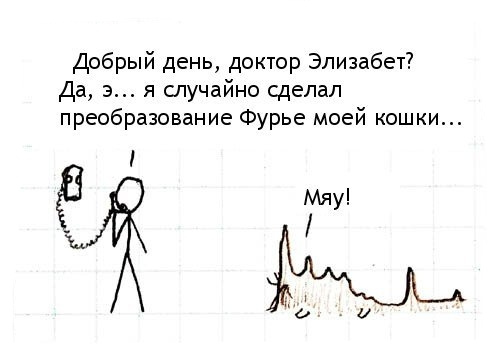
\includegraphics[width=\linewidth]{\imagesdir/comics_fourier.jpg}}
			\end{columns}
		}
	\end{frame}
	
	\begin{frame}
		\frametitle{Опции FFTW}

		\only<1>{
			\begin{center}
				$N = 512$
			\end{center}
			\begin{figure}[H]
				\begin{center}
					\begin{minipage}[h]{0.48\linewidth}
						\center{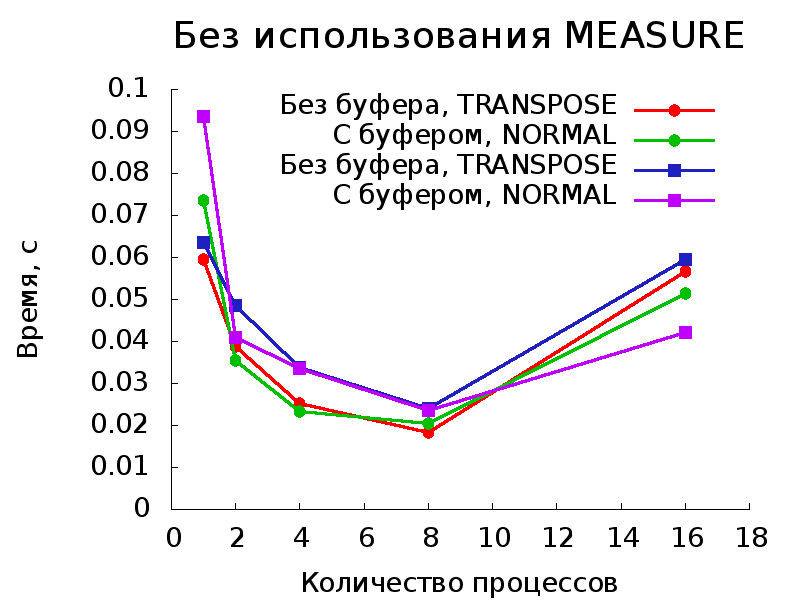
\includegraphics[width=0.95\linewidth]{\graphsdir/Skif/FFTW_compare_N512_nomeasure.png}} \\
					\end{minipage}
					\hfill
					\begin{minipage}[h]{0.48\linewidth}
						\center{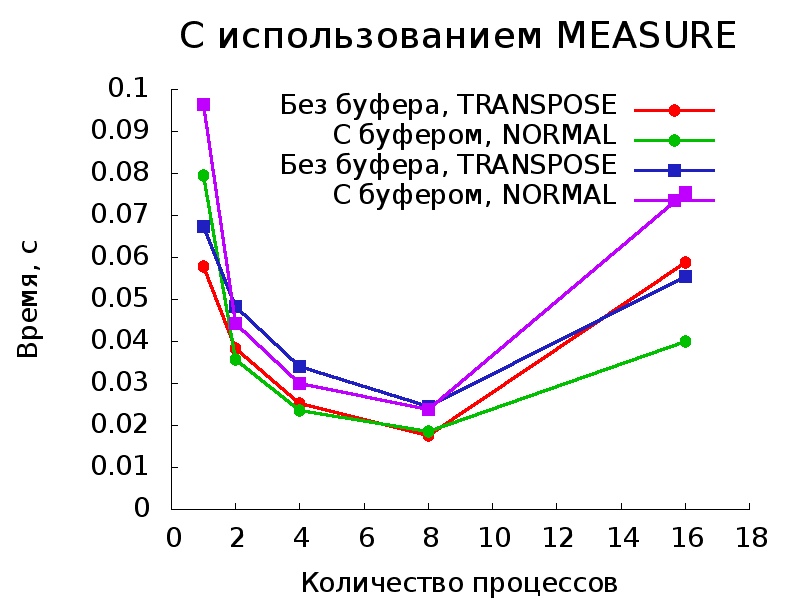
\includegraphics[width=0.95\linewidth]{\graphsdir/Skif/FFTW_compare_N512_measure.png}} \\
					\end{minipage}
				\end{center}
			\end{figure}
		}
		
		\only<2>{
			\begin{center}
				$N = 2048$
			\end{center}
			\begin{figure}[H]
				\begin{center}
					\begin{minipage}[h]{0.48\linewidth}
						\center{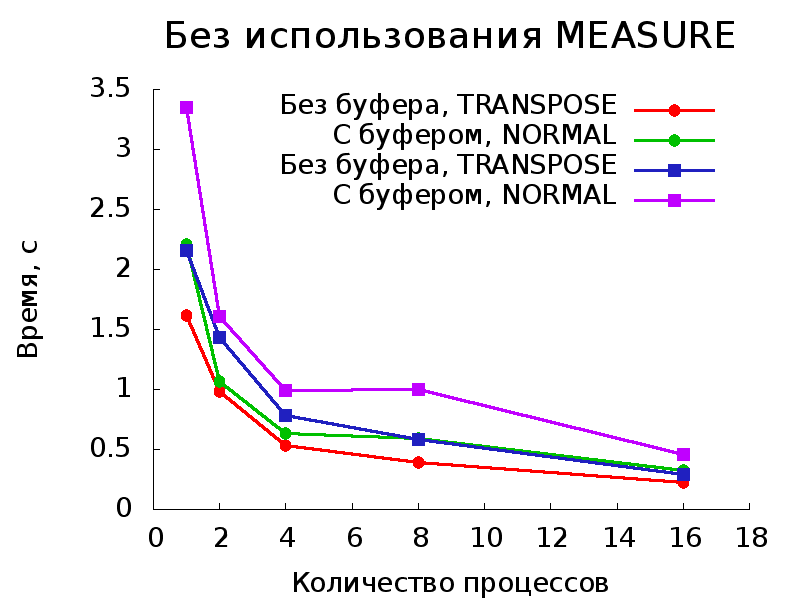
\includegraphics[width=0.95\linewidth]{\graphsdir/Skif/FFTW_compare_N2048_nomeasure.png}} \\
					\end{minipage}
					\hfill
					\begin{minipage}[h]{0.48\linewidth}
						\center{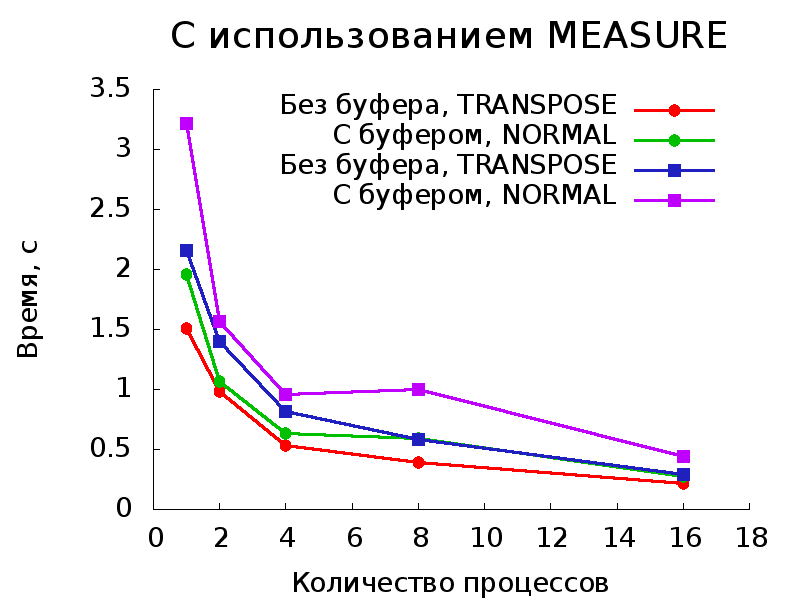
\includegraphics[width=0.95\linewidth]{\graphsdir/Skif/FFTW_compare_N2048_measure.png}} \\
					\end{minipage}
				\end{center}
			\end{figure}
		}
		
		\only<3>{
			\begin{center}
				$N = 8192$
			\end{center}
			\begin{figure}[H]
				\begin{center}
					\begin{minipage}[h]{0.48\linewidth}
						\center{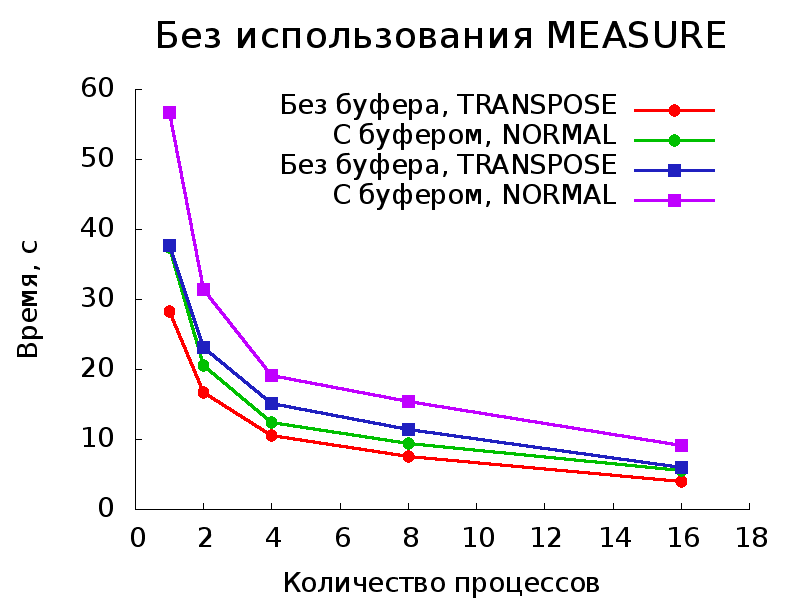
\includegraphics[width=0.95\linewidth]{\graphsdir/Skif/FFTW_compare_N8192_nomeasure.png}} \\
					\end{minipage}
					\hfill
					\begin{minipage}[h]{0.48\linewidth}
						\center{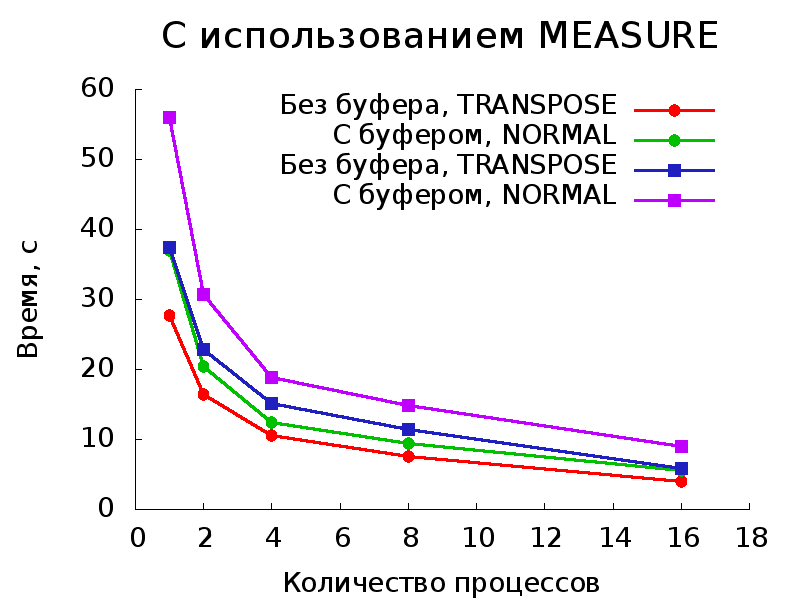
\includegraphics[width=0.95\linewidth]{\graphsdir/Skif/FFTW_compare_N8192_measure.png}} \\
					\end{minipage}
				\end{center}
			\end{figure}
		}
	\end{frame}
	
	\begin{frame}
		\frametitle{Минивывод: <<лучшее враг хорошего>>}

		Таким образом, обычно быстрее всего работает вариант без дополнительного буфера
		и с опцией FFTW\_TRANSPOSED\_ORDER, f использование дополнительно опции
		FFTW\_MEASURE не позволяет получить ощутимый прирост производительности.
		
		\vfill
		
		\begin{center}
			Зависимость времени такта от опций компиляции: \\
			\vskip1em
			\begin{tabular}{ | c | c | c | }
				\hline
				Опция		&	$np=8$	&	$np=16$ \\
				\hline
				\hline
				-O2	(по умолчанию)	&	9.0 с		&	5.0 с \\
				\hline
				\hline
				-О1		&	9.2 с	 	&	5.3 с \\
				\hline
				-О3		&	8.8 с		&	5.1 с \\
				\hline
				-Оs		&	9.0 с		&	5.2 с \\
				\hline
				-fast	&	8.9 с		&	5.2 с \\
				\hline
			\end{tabular}
		\end{center}
	\end{frame}
	
	\begin{frame}
		\frametitle{Результаты замеров времени для лучшего набора опций}
		
		\only<1>{
			\begin{center}
				Ускорение параллельной программы
			\end{center}
			\begin{figure}[H]
				\begin{center}
					\begin{minipage}[h]{0.48\linewidth}
						\center{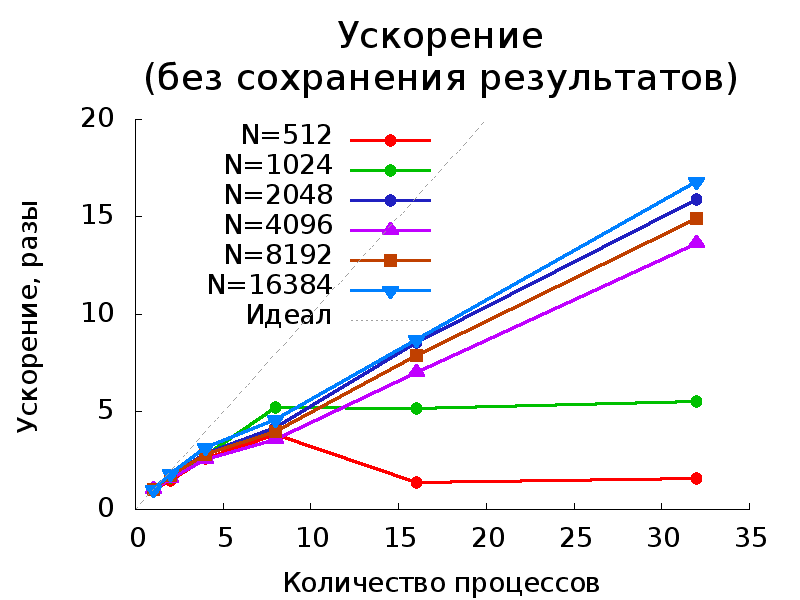
\includegraphics[width=0.95\linewidth]{\graphsdir/Skif/FFTW_acceleration_nosave.png}} \\
					\end{minipage}
					\hfill
					\begin{minipage}[h]{0.48\linewidth}
						\center{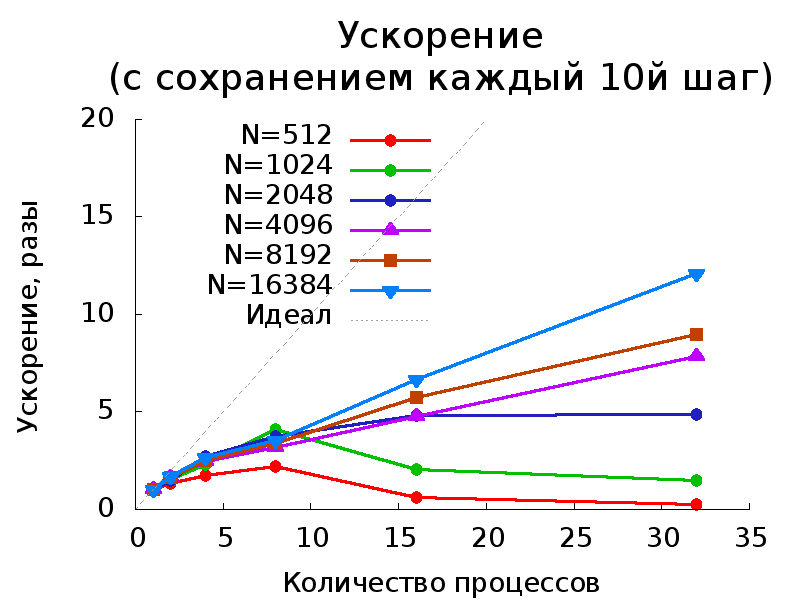
\includegraphics[width=0.95\linewidth]{\graphsdir/Skif/FFTW_acceleration_withsave.png}} \\
					\end{minipage}
				\end{center}
			\end{figure}
		}
		
		\only<2>{
			\begin{center}
				Эффективность параллельной программы
			\end{center}
			\begin{figure}[H]
				\begin{center}
					\begin{minipage}[h]{0.48\linewidth}
						\center{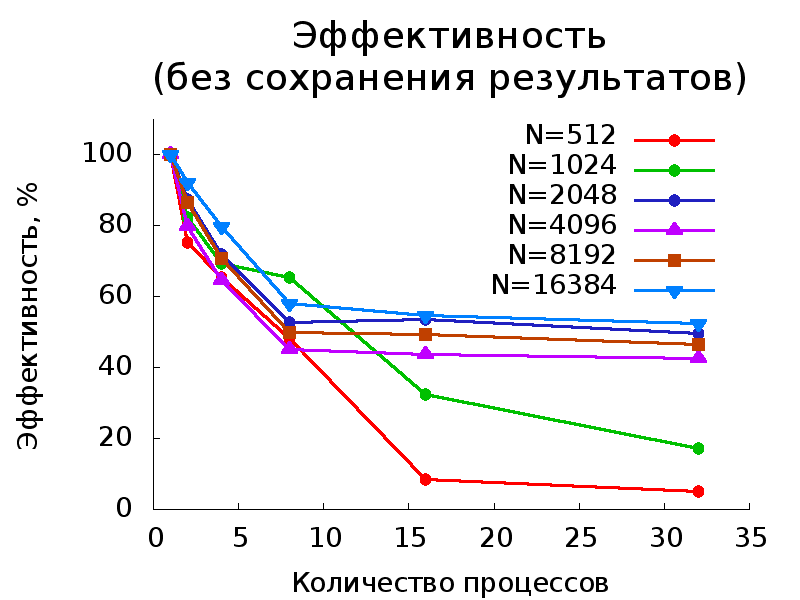
\includegraphics[width=0.95\linewidth]{\graphsdir/Skif/FFTW_efficiency_nosave.png}} \\
					\end{minipage}
					\hfill
					\begin{minipage}[h]{0.48\linewidth}
						\center{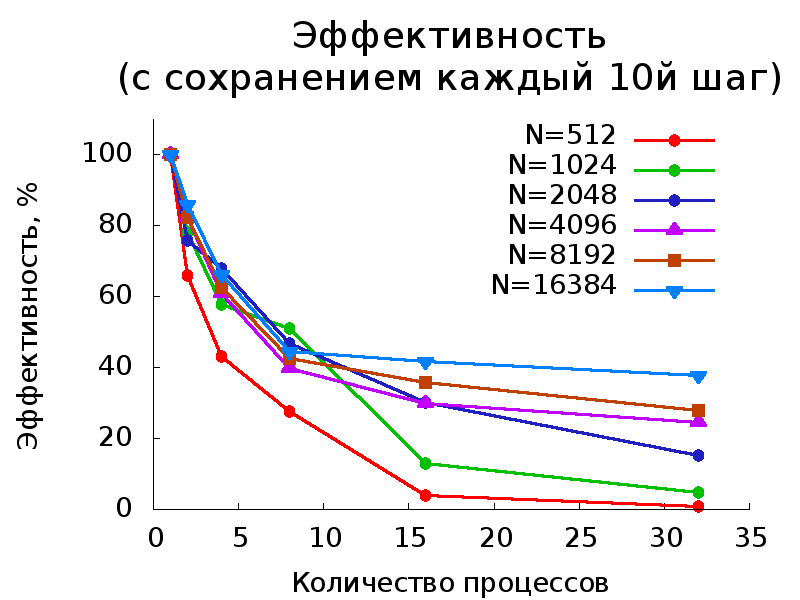
\includegraphics[width=0.95\linewidth]{\graphsdir/Skif/FFTW_efficiency_withsave.png}} \\
					\end{minipage}
				\end{center}
			\end{figure}
		}
	\end{frame}
	
	\subsection{Неявная схема: метод прогонки}

	\begin{frame}
		\frametitle{Неявная схема: метод прогонки}

		\only<1>{
			\begin{equation}
		    	\left\{
		    		\begin{aligned}
		        		2\textbf{i}\frac{h_1}{2}\frac{\hat{E}_{0,j}-E^k_{0,j}}{\Delta z} &= \frac{1}{2}\left(\frac{\hat{E}_{1,j}-\hat{E}_{0,j}}{h_1}\right) + \frac{1}{2}\left(\frac{E^k_{1,j}-E^k_{0,j}}{h_0}\right)\\
		        		2\textbf{i}\frac{h_{i+1}+h_i}{2}\frac{\hat{E}_{i,j}-E^k_{i,j}}{\Delta z} &= \frac{1}{2}\left(\frac{\hat{E}_{i+1,j}}{h_{i+1}} -\left(\frac{1}{h_{i+1}} + \frac{1}{h_i}\right)\hat{E}_{i,j} + \frac{\hat{E}_{i-1,j}}{h_i}\right) \\
		        		&\qquad+ \frac{1}{2}\left(\frac{E^k_{i+1,j}}{h_{i+1}} -\left(\frac{1}{h_{i+1}} + \frac{1}{h_i}\right)E^k_{i,j} + \frac{E^k_{i-1,j}}{h_i}\right)\\
		        		2\textbf{i}\frac{h_N}{2}\frac{\hat{E}_{N,j}-E^k_{N,j}}{\Delta z} &= \frac{1}{2}\left(\frac{\hat{E}_{N,j}-\hat{E}_{N-1,j}}{h_N}\right) + \frac{1}{2}\left(\frac{E^k_{N,j}-E^k_{N,j}}{h_{N-1}}\right) \nonumber
		    		\end{aligned}
		    	\right.
			\end{equation}

			Если шаг сетки равномерный, то есть $h_i=x_i-x_{i-1}=const$,
			то схема переходит в хорошо известную схему Кранка-Николсона.
		}
		
		\only<2>{
			\begin{figure}[H]
				\begin{center}
					\begin{minipage}[h]{0.48\linewidth}
						\center{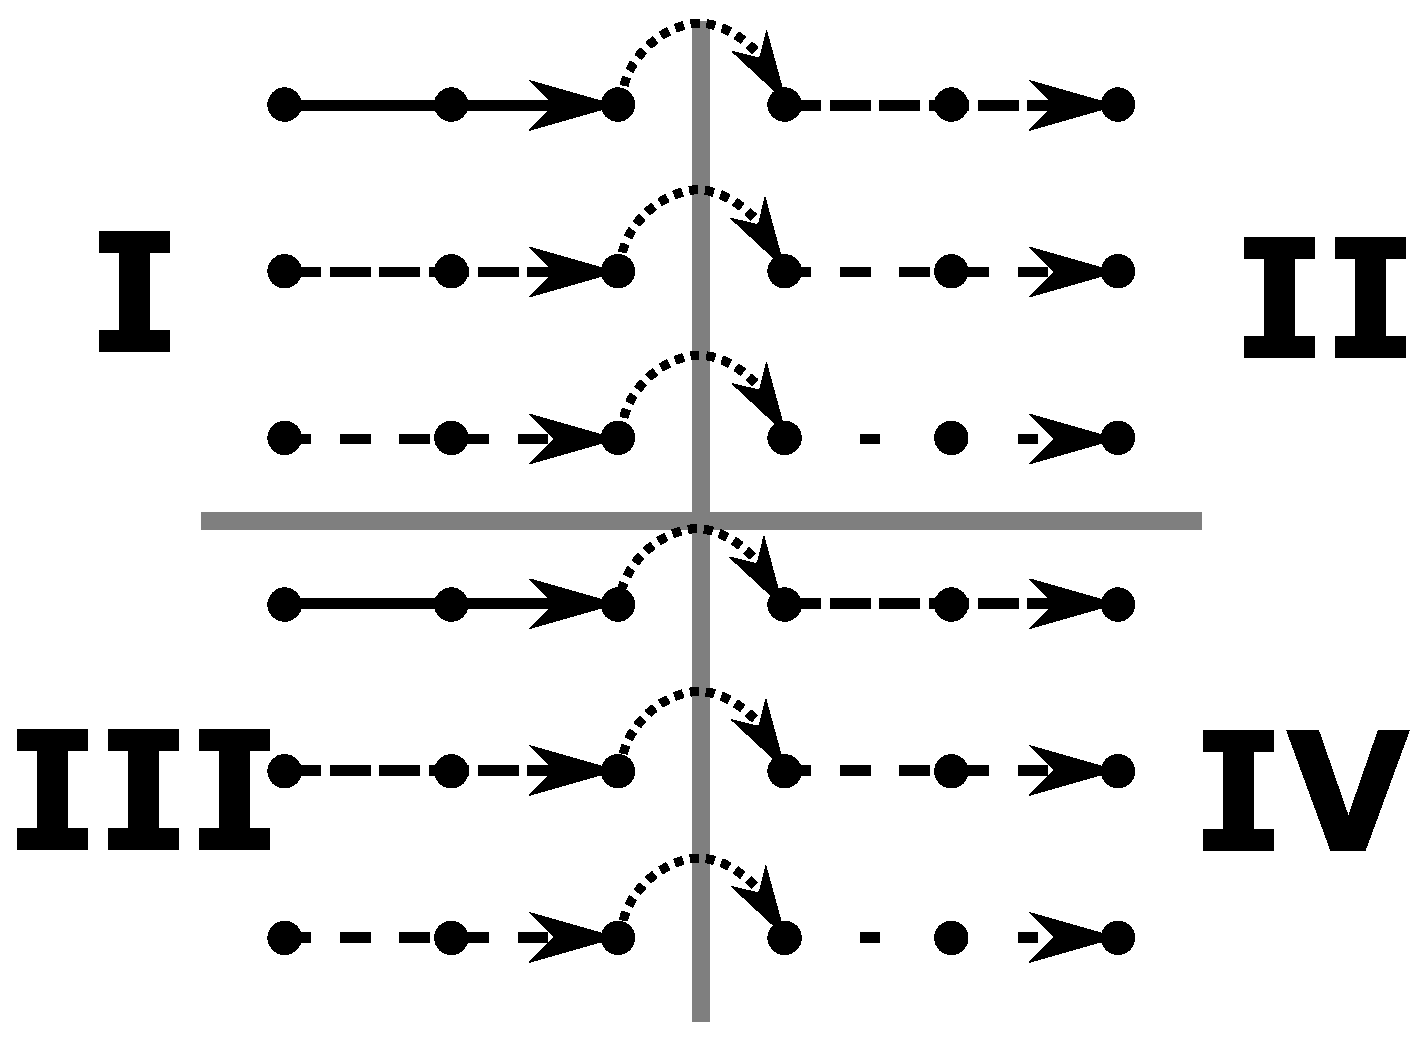
\includegraphics[width=0.95\linewidth]{\imagesdir/sweep_method_forward.eps}} \\
					\end{minipage}
					\hfill
					\begin{minipage}[h]{0.48\linewidth}
						\center{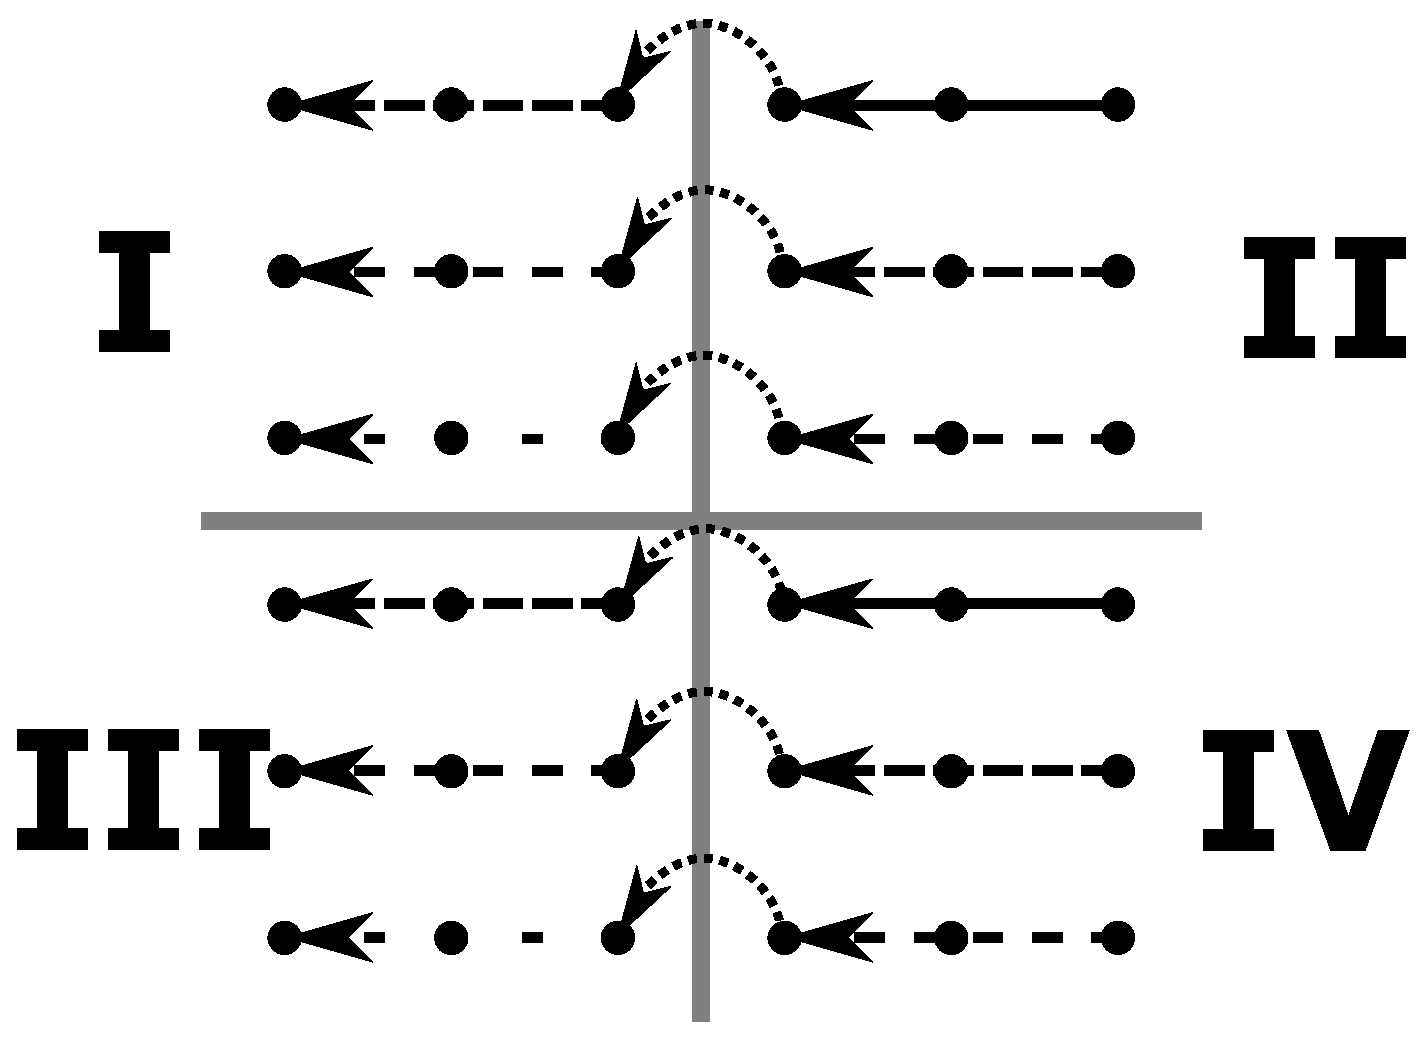
\includegraphics[width=0.95\linewidth]{\imagesdir/sweep_method_backward.eps}} \\
					\end{minipage}
				\end{center}
			\end{figure}
		}
	\end{frame}
	
	\begin{frame}
		\frametitle{Результаты замеров времени \\ СКИФ <<Чебышёв>>}
		
		\only<1>{
			\begin{center}
				Ускорение параллельной программы
			\end{center}
			\begin{figure}[H]
				\begin{center}
					\begin{minipage}[h]{0.48\linewidth}
						\center{\includegraphics[width=0.95\linewidth]{\graphsdir/Skif/Sweep_acceleration_nosave.png}} \\
					\end{minipage}
					\hfill
					\begin{minipage}[h]{0.48\linewidth}
						\center{\includegraphics[width=0.95\linewidth]{\graphsdir/Skif/Sweep_acceleration_withsave.png}} \\
					\end{minipage}
				\end{center}
			\end{figure}
		}
		
		\only<2>{
			\begin{center}
				Эффективность параллельной программы
			\end{center}
			\begin{figure}[H]
				\begin{center}
					\begin{minipage}[h]{0.48\linewidth}
						\center{\includegraphics[width=0.95\linewidth]{\graphsdir/Skif/Sweep_efficiency_nosave.png}} \\
					\end{minipage}
					\hfill
					\begin{minipage}[h]{0.48\linewidth}
						\center{\includegraphics[width=0.95\linewidth]{\graphsdir/Skif/Sweep_efficiency_withsave.png}} \\
					\end{minipage}
				\end{center}
			\end{figure}
		}
	\end{frame}
	
	\begin{frame}
		\frametitle{Результаты замеров времени \\ IBM Bluegene/P}
		
		\only<1>{
			\begin{center}
				Ускорение параллельной программы
			\end{center}
			\begin{figure}[H]
				\begin{center}
					\begin{minipage}[h]{0.48\linewidth}
						\center{\includegraphics[width=0.95\linewidth]{\graphsdir/Bluegene/Sweep_acceleration_nosave.png}} \\
					\end{minipage}
					\hfill
					\begin{minipage}[h]{0.48\linewidth}
						\center{\includegraphics[width=0.95\linewidth]{\graphsdir/Bluegene/Sweep_acceleration_withsave.png}} \\
					\end{minipage}
				\end{center}
			\end{figure}
		}
		
		\only<2>{
			\begin{center}
				Эффективность параллельной программы
			\end{center}
			\begin{figure}[H]
				\begin{center}
					\begin{minipage}[h]{0.48\linewidth}
						\center{\includegraphics[width=0.95\linewidth]{\graphsdir/Bluegene/Sweep_efficiency_nosave.png}} \\
					\end{minipage}
					\hfill
					\begin{minipage}[h]{0.48\linewidth}
						\center{\includegraphics[width=0.95\linewidth]{\graphsdir/Bluegene/Sweep_efficiency_withsave.png}} \\
					\end{minipage}
				\end{center}
			\end{figure}
		}
	\end{frame}
	
	
	\section{Заключение}
	
	\subsection{Основные результаты}

	\begin{frame}
		\frametitle{Основные результаты}
		
        \begin{itemize}
			\item Было проведено исследование работы 3х алгоритмов
				решения нелинейного уравнения квазиоптики: явной схемы с применением
				метода Рунге-Кутта 4-го порядка, неявной консервативной схемы,
				решаемой методом прогонки и метода с использованием БПФ.
			\item Выяснено, что явная схема обладает слишком большими требованиями
				к шагу интегрирования, что усложняет её применение в повседневных задачах.
				Среди оставшихся методом неявная схема лучше по масштабируемости,
				что на соответствуюшем кластере	может дать преимущество.
			\item Исследована зависимость времени расчёта БПФ с использованием
				библиотеки FFTW и найдены оптимальные значения опций.
			\item Выбор метода решения может определяться физической постановкой задачи.
		\end{itemize}
	\end{frame}

	\begin{frame}
		\begin{center}
			{\Huge \textbf{Спасибо за внимание!}}
		\end{center}
	\end{frame}
	
	\begin{frame}
		
		Авторы: \\
		\begin{equation*}
			\left\{
				\begin{array}{l}
					\text{Дергачёв А.\,А. <\href{mailto:dergachev88@yandex.ru}{dergachev88@yandex.ru}>} \\
					\text{Ефимов О.\,В. <\href{mailto:efimovov@yandex.ru}{efimovov@yandex.ru}>} \\
					\text{Сметанина Е.\,О. <\href{mailto:jannes-2002@yandex.ru}{jannes-2002@yandex.ru}>}
				\end{array}
			\right.
		\end{equation*}
		
		благодарят администрацию СКИФ МГУ <<Чебышёв>> за терпимость
		к~ночным загрузкам, администрацию IBM Blugene/P ВМиК МГУ
		за~предоставленные приоритеты и участников \url{http://xkcd.ru}
		за~добротный перевод комиксов.
		
		\vspace{2em}
		
		Исходный код работы доступен по адресу \\
		\url{https://github.com/Sannis/papers_and_talks/} \\
		Fork us on GitHub!
		
	\end{frame}
	
	\subsection{Содержание}
	
	\begin{frame}{Содержание}
		\vspace{1.0em}
		{\scriptsize \tableofcontents}
	\end{frame}

	\subsection{Дополнительные слайды}

	\begin{frame}
		\frametitle{Уравнение медленно меняющейся волны}
		
		\begin{eqnarray}
			2\textbf{i}k\frac{\partial E}{\partial z} =
			\left( 1-\frac{i}{\omega}\frac{\partial}{\partial t}\right)^{-1}\Delta_{\perp}E -
			k\frac{\partial^2 k}{\partial \omega^2}\frac{\partial E^2}{\partial t^2} +
			\frac{i}{3}k\frac{\partial^3 k}{\partial \omega^3}\frac{\partial^3 E}{\partial t^3} +  \nonumber \\
			+ \frac{2k^2}{n_0}\left[
				\left( 1-\frac{i}{\omega}\frac{\partial}{\partial t}\right)\Delta n_k +
				\left( 1+\frac{i}{\omega}\frac{\partial}{\partial t}\right)\Delta n_p
			\right] E  - i k \alpha E  \nonumber
		\end{eqnarray}
	\end{frame}


\end{document}

